\documentclass{article}

\usepackage{robust-externalize}
% Updates \graphicspath in compiled files to look for images in the root folder:
\robExtConfigure{latex support pictures}

% Automatically cache all tikz figures
% WARNING: read the "Bonus: how to cache all tikz pictures automatically" or you'll get into troubles
\cacheTikz
\cacheEnvironment{forest}{latex, add to preamble={\usepackage{forest}}}

\begin{document}

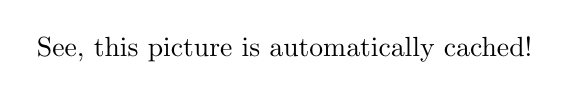
\begin{tikzpicture}
  \node[rounded corners]{See, this picture is automatically cached!};
\end{tikzpicture}

and this forest image is also automatically cached:
\begin{forest}
  [VP
    [DP]
    [V’
      [V]
      [DP]
    ]
  ]
\end{forest}
\end{document}
